
\chapter{Marco Teorico}

\section{Introducción}

Abordar un proyecto de robótica como Recurso Educativo Abierto (REA/OER), implica una serie de desarrollos conceptuales y teóricos que van a mas allá del diseño y desarrollo técnico de hardware y software. El uso de REA/OER \citep{montoya2012recursos} implica un compromiso ''político'' (entendiendo esto como una postura ideológica con respecto al uso de a tecnología) y la apropiación de términos conceptuales como ''software libre'' y ''soberanía tecnológica''. En este capitulo, se tratara de dar cuenta sobre los conceptos técnicos/teóricos para  la adopción de un proyecto de robótica educativa basado en software y hardware libre, tomando como base que la adopción de un proyecto de robótica educativa libre, implica adoptar las filosofías inherentes al software y la cultura libre.

\section{Soberanía tecnológica}

El concepto de soberanía tecnológica plantea una alternativa al proceso calificado por James \citet{boyle_second_2003} como el “segundo cercamiento de los bienes comunes”. Si la acumulación inicial del capital se produjo mediante el cerco (enclosure) de las tierras comunales, este segundo cerco a los bienes comunes pretende la apropiación privada, mediante el sistema de marcas registradas, patentes y las leyes de propiedad intelectual, de objetos e ideas que hasta ahora quedaban excluidos por considerarse bienes comunes inapropiables. En este contexto El uso de software libre sirve como empoderamiento para lograr, como dice Paulo \citet{freire_pedagogiautonomi:_2006}, una “pedagogía de la autonomía” , y no solo una base de usuarios cautivos para las empresas desarrolladoras de software. 

\section{Software libre}

El software libre es un movimiento que comenzó en el año 1983 cuando Richard \cite{stallman_software_2007} anuncio el proyecto GNU, como contra posición a la aparición de monopolios artificiales en el desarrollo de software \citep{beatriz_busaniche_argentina_2010}. Se podría decir que la meta del movimiento fue dar libertad a los usuarios de programas de computadoras remplazando el software con términos de licencias restrictivas (software privativo),  por una alternativa libre.

La comunidad de desarrolladores de software libre plantea que el software (para ser considerado libre) debe poder ser copiado, estudiado, distribuido y modificado libremente por cualquier persona o comunidad. En ese sentido, se vuelve de vital importancia poder contar con el código fuente (y no solo el código maquina o binario) de los programas para poder estudiarlos y modificarlos, ademas de tener una licencia (la licencia GNU/GPL) que proteja el derecho de autor y permita que ese código fuente pueda ser distribuido sin el peligro de que sea apropiado por alguien mas.

Por lo tanto para poder entender el concepto del software libre y la mirada política que hay detrás del movimiento, lo principal es poder entender los conceptos técnicos que implican el desarrollo de software y la diferencia entre el código binario (archivo ejecutable)  y el código fuente (escrito en un lenguaje de programación).

\subsection{Codigo fuente}

El software que diariamente usamos en nuestras computadoras esta compuesto por archivos  binarios, largas listas de ceros y unos (código binario) con los cuales la computadora lee y ejecuta las instrucciones que estos archivos les brindan. Originalmente, en el desarrollo de software, los ingenieros escribían directamente sobre la memoria de las computadoras de la época, grandes mainsframes que ocupaban habitaciones completas, pero con el crecimiento de la potencia de las computadoras, y la consiguiente complejidad en el desarrollo del  los programas que se necesitaban usar para controlar estas nuevas maquinas, se comenzó a ver la necesidad de contar con una forma mas eficiente y sencilla de poder crear programas para que una computadora. De esa época nace la idea un programa compilador que convirtiera la información escrita en un lenguaje formal (con cierto grado de aproximación a un lenguaje natural humano) y que pasara toda esa información a un lenguaje de maquina (código binario).

Un compilador es en su definición mas genérica un programa que toma como entrada un texto de un programa escrito en cierto lenguaje y produce como salida el texto de un programa en otro lenguaje \citep{grune_diseno_2007}, manteniendo el archivo original (código fuente) y el archivo de salida (código objeto, generalmente un archivo binario ejecutable por la computadora),  es decir que un compilador convierte  (o traduce como termino mas general) un archivo de código fuente a un archivo de código binario, permitiendo escribir en un lenguaje mas parecido al lenguaje natural (y mas sencillo de entender para los humanos).

   Por consiguiente podemos considerar a un lenguaje de programación como un lenguaje formal, donde una serie de instrucciones inequívocas conforman un algoritmo \citep{giro_lenguaje_2015}  que puede ser convertido por un compilador en un archivo de instrucciones binarias para ser ejecutado por una computadora.
   
Richard \cite{stallman_software_2007} hace la analogía entre el código fuente y una receta de cocina, donde uno siguiendo instrucciones sencillas y no ambiguas (los pasos para hacer una torta por ejemplo) puede llegar a obtener un producto final (la torta en este caso). De esa forma y en este esquema, la receta de cocina seria igual al código fuente y el producto final (la torta) seria igual al código binario (o ejecutable). Naturalmente si nosotros solo tenemos la torta, descubrir como obtener de vuelta la receta (ingeniería inversa) es mucho mas difícil que en el sentido inverso (receta-torta).

Haciendo un ejemplo mas concreto podemos ver las diferencias entre el software y el codigo fuente podemos ver la tabla1 propuesta por \cite{hart_open_2003}.

\begin{table}
\begin{center}
\begin{tabular*}{1\textwidth}{@{\extracolsep{\fill}} | l | l | } 
\hline
Lenguaje de programación & Código fuente  \\ \hline
ANSI C &
\begin{lstlisting}[language=C]
#include <stdio.h>
int main(int argc, char* argv[])
{
puts("Hola mundo!");
}
\end{lstlisting}
\\ \hline
Python &
\begin{lstlisting}[language=PYTHON]
print "hello world"
exit()
\end{lstlisting}
\\ \hline
binario                          & 01001000011001010110110001 \\
(''hello world'' en ASCII)       & 10110001101111001000000101 \\
                                 & 01110110111101110010011011 \\
                                 & 0001100100 \\ \hline
\end{tabular*}
\label{cod_fuente}
\caption{Lenguajes de programación, comparación entre código fuente y código máquina}
\end{center}
\end{table}

  
  
Como plantean Jordi \cite{adell_software_2007}, la facilidad de cambiar un programa escrito en python, por ejemplo, para que en ves de decir “Hello World” diga “Hola Mundo” seria bastante trivial y fácil de hacer, sin embargo para hacerlo desde código binario se vuelve muy complejo, y eso que solamente son los caracteres de la palabra “Hello World” no un programa completo el cuañ hasta el mas sencillo puede contener miles y hasta  millones de ceros y unos.

 Por tanto para un programador es necesario poder contar con el código fuente de un software para poder modificarlo, estudiarlo y comprender su funcionamiento (y que no sea solamente una caja negra).
 
Teniendo en cuenta estos conceptos, podemos explicar algunas de las definiciones que se utilizan sobre un software para poder ser considerado como software libre. Richard \cite{stallman_software_2007} define 4 “libertades” que tiene que tener dicho software para poder ser considerado como software libre:

\begin{itemize}
   \item libertad 0: La libertad de usar el programa, con cualquier propósito (Uso)
   \item libertad 1: La libertad de estudiar cómo funciona el programa y modificarlo, adaptándolo a las propias necesidades (Estudio).
   \item libertad 2: La libertad de distribuir copias del programa, con lo cual se puede ayudar a otros usuarios (Distribución).
   \item libertad 3: La libertad de mejorar el programa y hacer públicas esas mejoras a los demás, de modo que toda la comunidad se beneficie (Mejora).
 \end{itemize} 
 
Un programa es software libre si otorga a los usuarios todas estas libertades de manera adecuada. Por lo tanto el echo de contar con el código fuente es una condición necesaria para poder aplicar las 4 libertades que plantea la FSF (Free Software Foundation), lo dicho hasta aquí supone que todos los programas desarrollados y distribuidos bajo licencias libres (por ej. -la licencia GNU/GPL V3) tienen que se distribuidos con los archivos de código fuente ademas de de los archivos ejecutables (en el caso de programas compilados).

El software libre busca proteger las libertades individuales de los usuarios de computadoras como oposición a los desarrollos de software privativos (como los define la FSF), licencias restrictivas de uso, software malicioso (malwares, backtrack, etc.) monopolios \citep{beatriz_busaniche_argentina_2010}, y practicas poco éticas que algunas empresas pueden aplicar a sus usuarios de software. En cambio, gracias al software libre, los usuarios no están restringidos por el desarrollador de la aplicación y son dueños completos de el programa que necesitan usar, permitiendo a comunidades, organismos estatales y/o universidades, adaptar dicho software a las necesidades concretas de cada grupo, y así poder dar respuesta a necesidades puntuales que podrían no ser ''rentables'' para una empresa particular.

\begin{wrapfigure}{r}{0.5\textwidth}
%\begin{figure}[h]
  \begin{center}
    
\includegraphics[width=0.5\textwidth]{figuras/fsf.png}
    \caption{Logotipo del Free Software Foundation}
    \label{fig: }
  \end{center}
%\end{figure}
\end{wrapfigure}

Se podría decir que el software libre es un desarrollo soportado por las comunidades y para las comunidades, donde el esquema de desarrollo es distribuido y global, o como dice \citep{raymond_catedral_1998} un esquema donde el desarrollo de software libre es mas parecido a un ''bazar'' donde todos aportan de manera ''desorganizada'' y des centralizada, en contra posición a un desarrollo mas parecido a una ''catedral'', donde un arquitecto es el jefe central del desarrollo, en un esquema fuertemente estructurado.

\section{Hardware de especificaciones abiertas }

\begin{wrapfigure}{r}{0.5\textwidth}
  \begin{center}
    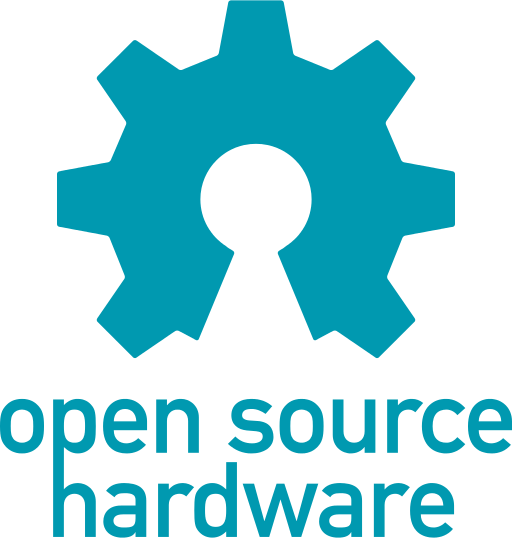
\includegraphics[width=0.2\textwidth]{figuras/Open-source-hardware-logo.png}
    \caption{Logotipo del Open Source Hardware}
    \label{fig: }
  \end{center}
\end{wrapfigure}

Por otro lado, el movimiento de hardware libre (o hardware de especificaciones abiertas) , busca llevar el concepto del software libre (la libertad de usar, estudiar, distribuir o mejorar el software) al diseño de  componentes físicos, especificando una licencia que permite distribuir planos y código fuente de desarrollos de PCBs y hardware electrónico. Asimismo, se considera que un diseño de circuito (esquematico, diseño de PCB y archivos GERBER) debe ser desarrollado con software libre y usando formatos abiertos.

Tomando la declaración de principios de la \textbf{Open Source Hardware association} \footnote{http://www.oshwa.org/definition/spanish/} , podemos decir que:

\begin{center}
\textit{
Hardware de Fuentes Abiertas (OSHW en inglés) es aquel hardware cuyo diseño se hace disponible públicamente para que cualquier persona lo pueda estudiar, modificar, distribuir, materializar y vender, tanto el original como otros objetos basados en ese diseño. Las fuentes del hardware (entendidas como los ficheros fuente) habrán de estar disponibles en un formato apropiado para poder realizar modificaciones sobre ellas.
}
\end{center}


\begin{wrapfigure}{r}{0.5\textwidth}
  \begin{center}
    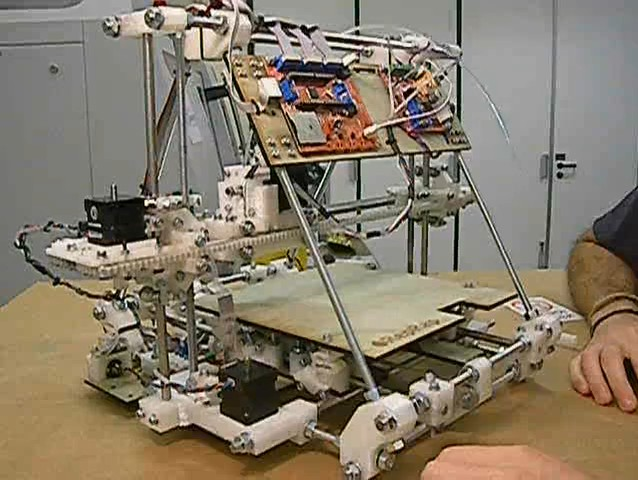
\includegraphics[width=0.2\textwidth]{figuras/reprap.jpg}
    \caption[Caption for LOF]{Impresora 3d diseñada con hardware libre}
       
    \label{fig:reprap }
  \end{center}
\end{wrapfigure}

%\footnote{By CharlesC - http://vimeo.com/6865848 - video from open-source RepRap project, CC BY-SA 3.0, https://commons.wikimedia.org/w/index.php?curid=8020149}

Idealmente, el hardware de fuentes abiertas debería ser diseñado para poder utilizar componentes, materiales y herramientas de alta disponibilidad y fácil acceso (en lo posible), utilizando herramientas de fuentes abiertas (en el caso del software de desarrollo), permitiendo de esa forma maximizar la posibilidad de construir y usar ese hardware por parte de los usuarios. 

Es importante notar como la OSHW plantea que un hardware para ser considerado de estándares abiertos, no solo deben ser distribuido sus planos y esquemáticos con un formato libre, si no que ademas poder permitir a sus usuarios la posibilidad concreta de fabricar ese mismo hardware. El hardware de fuentes abiertas da libertad de controlar la tecnología y al mismo tiempo permite compartir conocimientos.

\citet{gonzalez_hardware_2003} plantean una clasificación del hardware en función de su diseño y el software empleado para su creación, definiendo una clasificación primaria de los 3 tipos de archivos necesarios para la fabricación de un PCB (Printed Circuit Board por sus siglas en ingles), el \textit{esquemático},el archivo de  \textit{pcb} y el archivo \textit{GERBER}. En función de esa clasificación, se puede separar al hardware en tres tipos de clasificación:

\begin{itemize}
   \item (P): Software de diseño propietario.
   \item (L): Software de diseño libre.
   \item (M): Software de diseño propietario pero multi plataforma (funciona en sistemas operativos libres y tambien en propietarios)
 \end{itemize} 

Por tanto los tres archivos de construcción para el circuito electrónico, pueden ser de clasificación como enteramente libres (tipo \textbf{LLL}) o completamente propietarios (\textbf{PPP}), y todas sus combinaciones posibles.


\subsection{Software libre en la escuela}

\citet{adell_software_2007} consideran al Software libre una alternativa para aplicar en el contexto del aula por sus ventajas pragmáticas (menor o hasta incluso nulo costo por licencias) que permiten ahorrar presupuesto, y por sus valores ético, políticos y sociales \citep{hart_open_2003}, que funcionan como disparadores de discusiones sobre los valores que una institución educativa tendría que promover.El software libre en la educación trata sobre la libertad de los docentes y dicentes, porque Como dice Paulo \citet{freire_pedagogioprimido._2015}: \textit{''Nadie libera a nadie, ni nadie se libera solo. Los hombres se liberan en comunión''}.

La incorporación del software libre en el desarrollo curricular del aula, promueve la cooperación entre las personas donde el software privativo la convierte en un delito \cite{adell_software_2007}, el software libre permite a las instituciones escolares sumar sus esfuerzos académicos a un proyecto global, independiente de los vaivenes económicos de las grandes corporaciones, y adaptable a las necesidades concretas de la comunidad donde ese establecimiento esta asentado y que puede no ser rentable para una compañía adaptar su software para esas realidades concretas.

Usando software libre, los alumnos pueden disponer de copias gratuitas de los programas que necesiten para el trabajo escolar, sin restricciones de licencias que obligan a tener un software de menor calidad para ''obligar'' a los usuarios a comprar las versiones ''completas''. Al disponer del código fuente, se puede adaptar a las necesidades del docente para situaciones concretas, como traducir dicho software a el idioma de sus alumnos (como el caso de la traducción de la suite ofimática Libreoffice al idioma aimara\footnote{http://www.elmundo.es/navegante/2007/08/03/tecnologia/1186167876.html}). 

Los proyectos de software libre suelen tener un coste inicial de desarrollo muy bajo \citep{adell_software_2007}, generalmente empiezan como un desarrollo personal de algún programador o pequeño grupo de entusiastas, y gracias al trabajo global y distribuido logra crecer y obtener una ''masa critica'' de desarrolladores que lo hacen crecer, o como menciona \cite{boyle_second_2003}

\begin{center}
\textit{en una red global hay tanta gente y los costos son tan bajos que incluso los proyectos relativamente complejos atraen a las personas motivadas y capaces cuyo precio base ya ha sido superado}
\end{center}

 de esa forma proyectos muy complejos pueden ver la luz, y ese mecanismo puede ser aprovechado por los colegios para ser generadores de contenido que pueda ser aprovechados por otras instituciones.

\section{Robots}

A nivel histórico, la palabra robots viene definida por la la obra R.U.R. (Robots Universales Rossum) del dramaturgo checo Karel Čapek, donde se uso por primera ves la expresión "robotnik" para referirse a seres humanos sintéticos creados para ser esclavos de la humanidad  \citep{zabala_robotica_2007}. Sin embargo la popularidad del termino robot se da por el escritor y divulgador científico Isaac Asimov, que uso el termino robótica para referirse a la disciplina que estudia a sistemas autónomos con cierto grado de capacidad para tomar decisiones e interaccionar con su medio (físico o virtual).

Se podría decir que cualquier sistema que posea sensores, actuadores y algún tipo de dispositivo que le permita realizar algoritmos de procesamientos, es un robot. Una definición tan laxa haría que prácticamente cualquier dispositivo pueda ser considerado un robot. Podemos decir entonces, que hay múltiples definiciones de la palabra robot, en función de las necesidades especificas de cada país u organización, por ejemplo si tomamos la definición empleada por la R.I.A \footnote{https://www.robotics.org/}, un robot (sobre todo pensando en el robot industrial) es\footnote{https://definitions.uslegal.com/r/robotics/} : 
  

\begin{center}
\textit{A robot is a reprogrammable, multifunctional manipulator designed to move material, parts, tools or specialized devices through variable programmed motions for the performance of a variety of tasks.}
\end{center}

lo que se podría traducir como: ''un robot es un manipulador multifuncional y reprogramable diseñado para desplazar materiales, componentes, herramientas o dispositivos especializados por medio de movimientos programados variables con el fin de realizar tareas diversas''.

Por otro lado, la J.A.R.A\footnote{http://www.jara.jp/e/index.html} (Japan Robot Association, ex J.I.R.A) usa una definición menos orientada a los manipuladores industriales (como los brazos robots que se usan en la industria automotriz) \citet{reyes_cortes_robotica:_2011}:

\begin{center}
\textit{Los robots son dispositivos capaces de moverse de modo flexible análogo al que poseen los organismos vivos, con o sin funciones intelectuales, permitiendo operaciones en respuesta a las órdenes humanas}
\end{center}




\section{Robótica educativa}
\citet{seymour_papert_desafio_1987} Desarrollo la teoría pedagógica del \textit{Construccionismo} la cual promueve la utilización de computadoras como recurso para apoyar el desarrollo de nuevas maneras de pensar y aprender. Papert plantea que La única habilidad competitiva a largo plazo es la habilidad para aprender, por lo tanto su enfoque metodológico esta orientado a usar las computadoras como herramientas para posibilitar ese desarrollo cognitivo en los alumnos. \citet{sanchez_robotica_2012} dicen que el construccionismo es reconocido como una teoría educativa que fundamenta el uso de la tecnología digital en educación.

En cuanto al uso de robótica como recurso educativo, \citet{sanchez_robotica_2012} dicen que por su carácter multidisciplinario, la robótica es una herramienta interesante para el uso como recurso facilitador del aprendizaje y el desarrollo de competencias generales, dado que Permite trabajar transversalmente múltiples disciplinas, y sirve como motivador para que los discentes lleven a cabo proyectos donde puedan experimentar y desarrollar sus actitudes cognitivas,como dice \citet{pitti_experiencias_2010}, la robótica es una herramienta construccionista. 
 
Por otro lado uno de los mayores problemas de la implementación de la robótica en el aula, es la gran carga de contenido técnico que debe afrontar el docente para poder trabajar con su curricula, en ese sentido varios fabricantes diseñaron Kits para el uso de robótica con fines educativos, sin embargo estos kits de robótica, generalmente,  son extremadamente caros y por lo tanto restrictivos para su utilización masiva por parte de los docentes. El coste operativo de implementar un kit de robótica comercial puede ser prohibitivo para colegios de pocos ingresos, pero también el costo de mantenimiento (reparación y remplazo de piezas defectuosas, actualizaciones etc.) termina siendo un factor clave a la hora de usar los robots como herramientas pedagógicas, a causa del ''peligro'' de que los alumnos rompan los robots y reponerlos salga tan caro como comprar un kit nuevo.

Por lo tanto, la Robótica educativa con software y hardware libre es una opción mas que viable para la aplicación en el proceso de aprendizaje, 
porque permite a las escuelas adaptar la tecnología a las necesidades especificas de la institución, permitiendo reutilizar componentes que se encuentren en el colegio ( aportados por la comunidad escolar), reciclando y asi ahorrar costos, a su ves por la gran expectativa que genera en los alumnos (y docentes), y al ser de código fuente libre, permite romper barreras culturales y políticas que pueden ir en detrimento de la calidad educativa, barreras como el alto costo de adquisición de los elementos, licencias privativas para el software de control o la falta de documentación especifica para comunidades minoritarias (traducciones a idiomas que no son viables comercialmente por ejemplo). La robótica educativa con software y hardware libre permite aprovechar las ventajas que ofrecen la filosofía de desarrollo que existe en las comunidades de software libre, donde ''mil ojos ven mas que uno'' \citet{raymond_catedral_1998}, permitiendo involucrar a la comunidad escolar en su conjunto y donde las soluciones aportadas por el grupo podran ser utilizadas en otros colegios y vice versa, generando una situaciones donde todos los involucrados salen favorecidos.

\section{Construccionismo}

El construccionismo es una teoría del aprendizaje diseñada por Seymour \cite{seymour_papert_desafio_1987} donde se resalta la importancia de la acción como parte principal en el proceso de aprendizaje. Toma como inspiración las ideas de la psicología construtivista partiendo del supuesto de que el conocimiento debe ser construido por el propio sujeto, el cual aprende a través de la acción, por lo tanto no es algo que se pueda solamente transmitir.

\begin{wrapfigure}{r}{0.5\textwidth}
  \begin{center}
    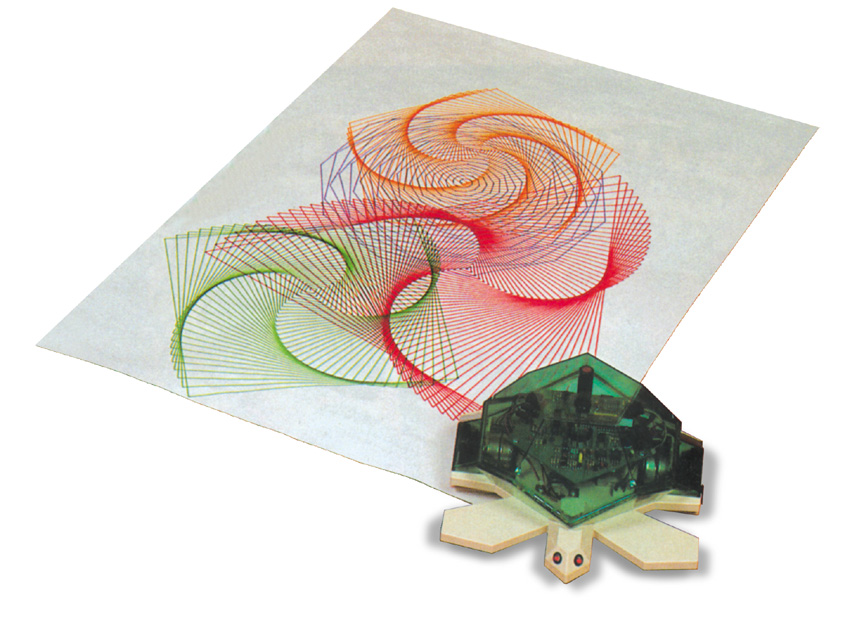
\includegraphics[width=0.2\textwidth]{figuras/Turtle_draw.jpg}
    \caption[Caption for LOF]{robot ''tortuga'' de la empresa Valiant}
    
    \label{fig:turtle }
  \end{center}
\end{wrapfigure}

% \footnote{By Valiant Technology Ltd., CC BY-SA 3.0, https://commons.wikimedia.org/w/index.php?curid=19501049}

El concepto central dentro del construccionismo radica en plantear actividades de confección y construcción de artefactos (aunque no necesariamente artefactos físicos) los cuales funcionan como facilitadores del aprendizaje porque los sujetos al construir un dispostivo (un robot, un castillo o un programa de computadora), construyen también sus propias estructuras de conocimiento. Papert afirma que los sujetos ademas, deben construir objetos que sean de su interés personal, para poder interesarse mas en el proceso de construcción (y por ende, en su proceso de construcción del conocimiento) al mismo tiempo que los objetos construidos ofrecen la posibilidad de hacer mas concretos, palpables y visibles (dentro del esquema de pensamiento del sujeto) los conceptos abstractos o teóricos, y por tanto, los hace más fácilmente comprensibles.

\cite{seymour_papert_desafio_1987}  da el ejemplo de los ''engranajes'' que tanto lo fascinaron en su infancia para plantear como pensar en un ''objeto con el cual pensar'', y como en el hecho de ''pensarse como un engranaje'' le permitió aprender conceptos formales matemáticos que forman parte del desarrollo de un sistema de engranajes (relación entre dientes y fuerza en un tren de engranajes por ejemplo).

\subsection{Lenguaje LOGO}

Como parte del Construccionismo, Papert desarrollo el lenguaje LOGO, un lenguaje formal \citet{giro_lenguaje_2015} diseñado para poder trabajar conceptos de matemáticas sobre la idea de interaccionar con una ''tortuguita'' que dibuja en función de las ordenes (algoritmo) que los alumnos escriben en la computadora.

\begin{wrapfigure}{R}{0.5\textwidth}
  \begin{center}
    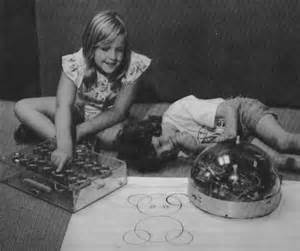
\includegraphics[width=0.2\textwidth]{figuras/logo_robot.jpg}
    \caption[Caption for LOF]{robot 'tortuga' original diseñado por el M.I.T}
    
    \label{fig:tortuga_mit}
  \end{center}
\end{wrapfigure}
El lenguaje LOGO esta diseñado para ser sencillo de aprender, con instrucciones (''primitivas'' en el argot LOGO) que son intuitivas para el usuario (la palabra 'adelante', hace que la tortuga avance N pasos,  al igual que ''atrás'' hace que retroceda) y sin embargo sigue siendo un lenguaje de programación completo y capas de hacer lo mismo que otros lenguajes de propósito general  (como C, FORTRAN u otros lenguajes de la época). Una de las ventajas de LOGO es su facilidad de poder hacer ''algo'' con muy pocas lineas de código (tipicamente algun dibujo con la ''tortuguita''), \cite{seymour_papert_desafio_1987} plantea que cualquier niño, bajo las condiciones adecuadas, puede aprender un lenguaje de programación.

Originalmente, las primeras pruebas de LOGO se hicieron con robots como el de la figura \ref{fig:tortuga_mit}, el cual estaba pensado para ser robusto, y capaz de soportar hasta el peso de un niño encima, las computadoras de la época no tenían capacidad de procesar gráficos de alta definición (y las impresoras eran caras y de uso casi exclusivo en las empresas), por lo tanto la ventaja de un robot eran muy interesantes.

\begin{wrapfigure}{R}{0.5\textwidth}
  \begin{center}
    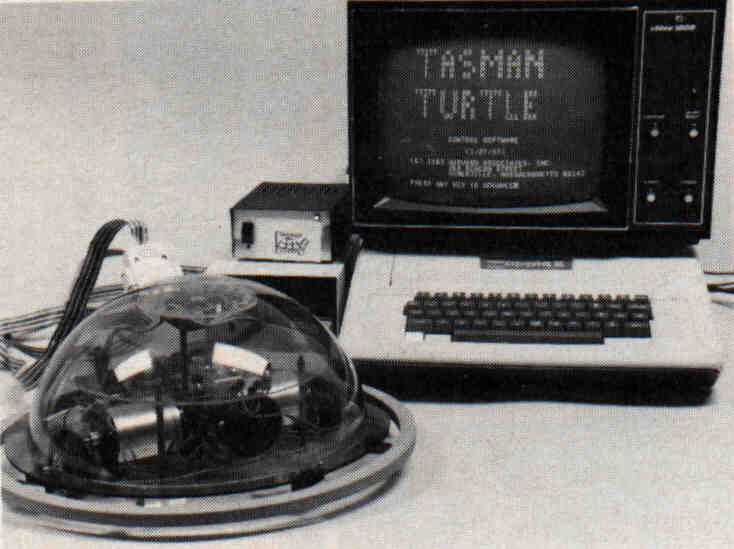
\includegraphics[width=0.2\textwidth]{figuras/turtle_with_apple.JPG}
    \caption[Caption for LOF]{Version 'mini' del robot tortuga controlado por un micro computador Apple}
    
    \label{fig:tortuga_2}
  \end{center}
\end{wrapfigure}

Con el advenimiento de las micro computadoras (como las ZX spectrum y las commodores C64), que contaban con la capacidad de trabajar  en monitores a color (o en los televisores CRT de la época) y con un bajo costo de adquisición, se dejo de utilizar los robots tortuga, para directamente trabajar con el lenguaje de programación LOGO y una ''tortuga virtual'', menos llamativa pero mucho mas barato de adquirir para los colegios.

\section{Lenguajes formales}

Podemos definir a un lenguaje formal como un lenguaje cuyos símbolos (alfabeto) y reglas para unir esos símbolos (gramática) están formalmente definidos \citep{giro_lenguaje_2015}. Por consiguiente se pordia decir que su particularidad  es la de un lenguaje cuyos significados son ''vacíos'', dicho en otros términos: en los lenguajes formales los signos pueden ser manipulados sin interpretación, se trata de un ''usar sin necesidad de entender'' para potenciar y mejorar los razonamientos en la medida que se evitan los sesgos cognitivos asociados al uso del lenguaje natural.

Un lenguaje de programación es un lenguaje formal, como la lógica y la matemática, con la diferencia que fue diseñado para realizar procesos que pueden ser llevados a cabo por computadoras (maquinas de Turing). Entre sus características principales, se encuentra la posibilidad de poder crear programas que gobiernen el comportamiento de una computadora, tanto a nivel físico (hardware) como lógico (software), por lo que son de suma importancia para generar algoritmos que permitan el control de una computadora.

En la primera época de las computadoras (las grandes mainframes como la ENIAC) estas eran programadas directamente escribiendo ''ceros y unos'' sobre su memoria, utilizando directamente lo que se define como \textbf{lenguaje de maquina}, o usando una serie de reglas nmemo técnicas que se dio a llamar como \textbf{lenguaje ensamblador}. La gran dificultad de programar software cada ves mas complejo hizo que se desarrollaran lenguajes de programación cada ves mas alejados del lenguaje de maquina y mas cerca del lenguaje natural, se dice comúnmente que un lenguaje de bajo nivel es aquel que se asemeja mas a la forma de trabajar de una computadora (assembler por ejemplo), y que un lenguaje de alto nivel, trata de ser mas parecido al lenguaje que usamos los seres humanos (python por ejemplo) y por lo tanto es mas fácil de entender para los programadores y para impartir cursos de iniciación a la programación \citep{de2016introduccion}.

\subsection{python}


\begin{wrapfigure}{r}{0.5\textwidth}
  \begin{center}
    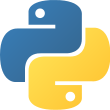
\includegraphics[width=0.2\textwidth]{figuras/Python-logo.png}
    \caption[Caption for LOF]{Logotipo de PYTHON}
    
    \label{fig:python_logo}
  \end{center}
\end{wrapfigure}

Python es un lenguaje de programación interpretado, de alto nivel y multi paradigma, cuya filosofía hace hincapié en una sintaxis que favorezca un código fácil de leer para los programadores. Por lo tanto y como dice \cite{marzal2003aprender}, python es un lenguaje ideal para la enseñanza de programación porque tiene una \textit{sintaxis} que facilita la economía de símbolos auxiliares (como el símbolo '';'' usado para indicar el final de linea en lenguaje C), es \textit{expresivo} (entendiendo esto como su capacidad para decir mucho con pocas lineas de código), y su \textit{semántica} es elegante, haciendo que sea fácil de entender y escribir.
